\subsection{Mixing of the latent Gaussian field}\label{sec:field-mixing}

The archived fits retain coefficient draws and running cell summaries, but no trajectories of $g$. We therefore replayed the four full-data chains for the tail-down model at $r=800$~km, using the revised code and the same 8,000-sweep schedule, 2,000-sweep burn-in, seeds and initial widths as the archived analysis. The field starts at zero in every chain; the initial widths are 10, 20, 40 and 80~km. The monitoring records values after both field colours have been updated, without changing proposals or random-number draws. Retained parameter draws agree with the archive to within $1.3\times10^{-14}$, and the stored cell summaries agree exactly.

We selected 128 vertex IDs at evenly spaced positions in the sorted list of vertices touching the survey footprint, and 32 from its complement, before inspecting their trajectories. We also recorded cell-length-weighted averages of the interpolated field over the whole network, the survey footprint, and its northern and southern halves, together with the north--south difference. The halves are defined by the median latitude of footprint cells. Diagnostics use all 6,000 retained states per chain, giving 24,000 stored draws for each monitored quantity; these coordinates and summaries do not exhaust all 145,329 field dimensions.

The broad field summaries mix poorly: their rank-normalized $\widehat R$ values range from 1.63 to 2.25, with bulk ESS estimates between 5.0 and 6.7 (Table~\ref{tab:field-mixing}). For the survey-footprint mean, the average within-chain autocorrelation is 0.999 at lag one and 0.896 at lag 100. The traces in Figure~\ref{fig:field-mixing} show persistent drift and disagreement, so these small ESS values are diagnostic warnings rather than a basis for precise Monte Carlo uncertainty estimates.

Local coordinates also show substantial dependence: among the 128 monitored footprint vertices, the median $\widehat R$ is 1.136, the maximum is 1.564, and 127 exceed 1.01; median bulk ESS is 21.7. Outside the footprint, 31 of the 32 monitored vertices exceed 1.01. Consequently, the field diagnostics support the earlier warning about incomplete posterior exploration, including spatial averages that can mix much more slowly than an individual coordinate. All fields were initialized at zero, so this check does not establish robustness to dispersed field starts.

The small conditional blocks provide a plausible mechanism for slow movement on large spatial scales, while dependence between the field, site counts, breeding coefficients and dispersal width may also contribute. These runs do not separate those causes or compare alternative samplers; larger-scale or joint updates would require their own empirical mixing assessment.


\begin{table}[H]
\centering\small
\caption{Latent-field diagnostics for the additional tail-down 800~km run. ESS is calculated across four chains; autocorrelations at lags 1 and 100 are averaged over the four within-chain estimates. The last row selects the largest $\widehat R$ among the 128 monitored footprint vertices.}
\label{tab:field-mixing}
\begin{tabular}{lrrrrr}
\toprule
Field quantity & $\widehat R$ & Bulk ESS & Tail ESS & ACF(1) & ACF(100)\\
\midrule
Whole-network mean & 2.249 & 5.0 & 21.2 & 0.998 & 0.839 \\
Survey-footprint mean & 1.703 & 6.3 & 13.8 & 0.999 & 0.896 \\
Northern mean & 1.998 & 5.4 & 11.6 & 0.999 & 0.882 \\
Southern mean & 1.629 & 6.7 & 20.3 & 0.999 & 0.865 \\
North--south contrast & 1.642 & 6.6 & 46.9 & 0.998 & 0.817 \\
Largest local $\widehat R$ & 1.564 & 7.3 & 18.3 & 0.954 & 0.536 \\
\bottomrule

\end{tabular}
\end{table}

\begin{figure}[htbp]
\centering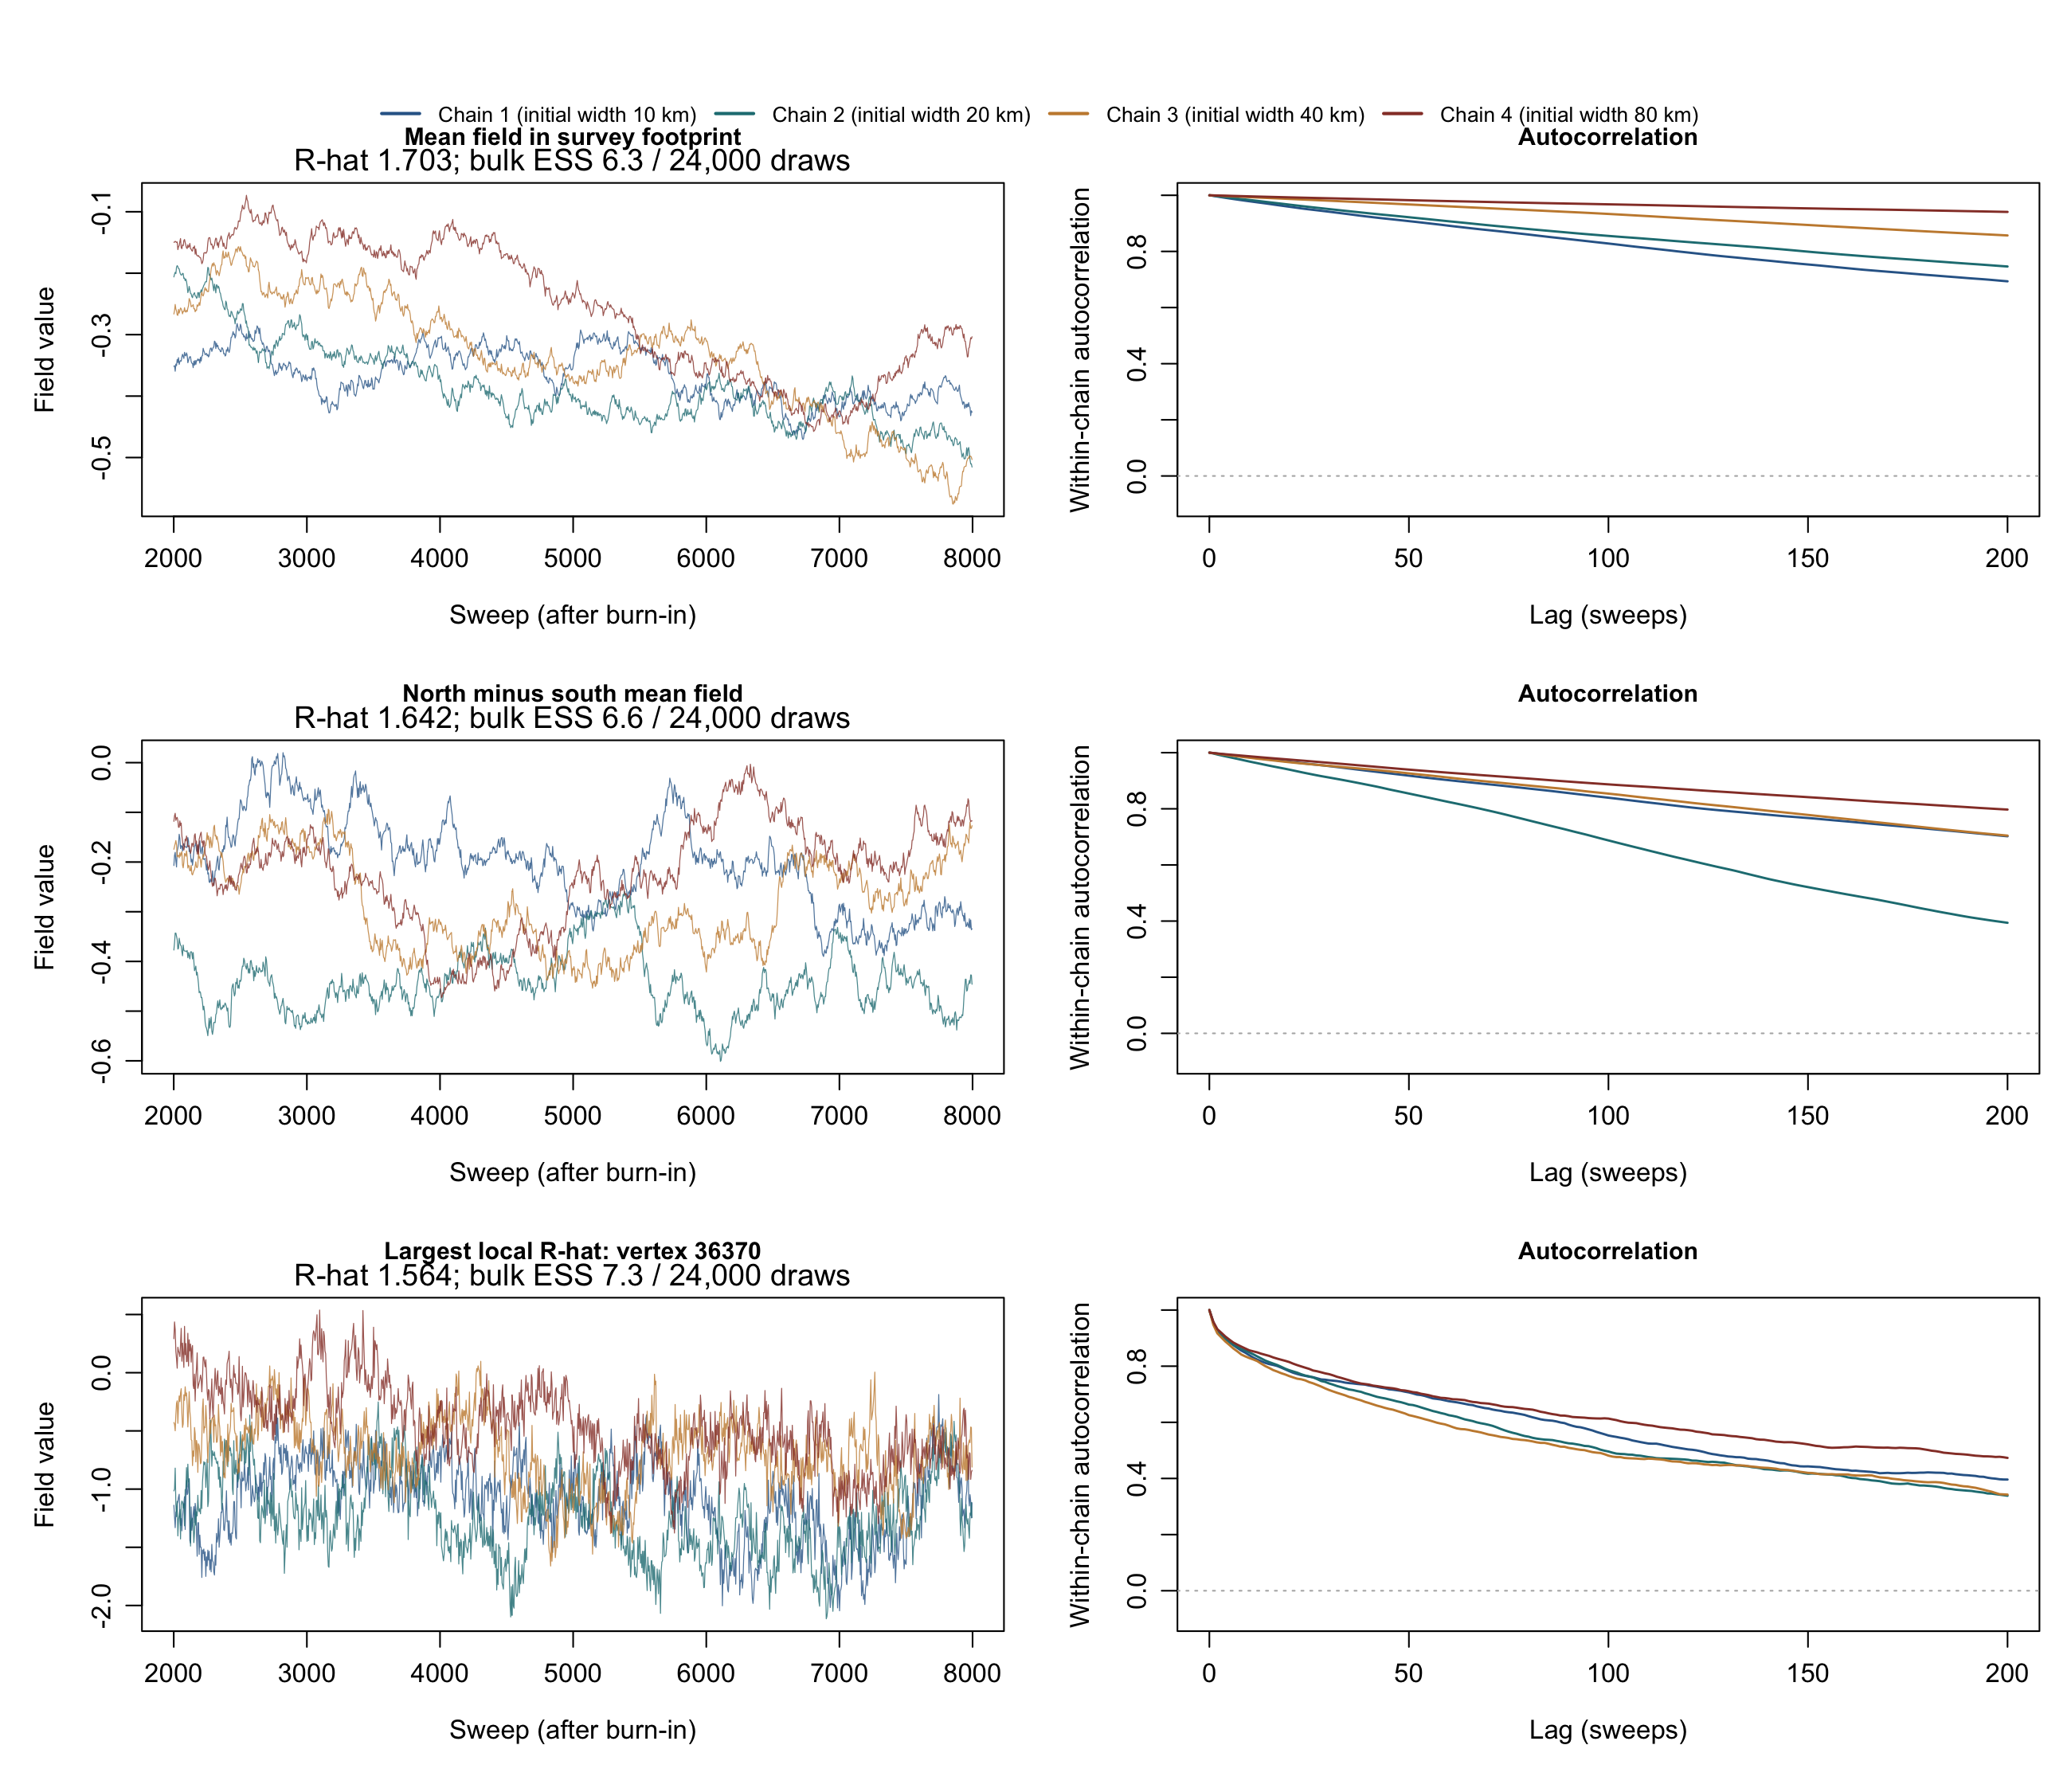
\includegraphics[width=\textwidth]{field_mixing.png}
\caption{Retained field traces and within-chain autocorrelations for the survey-footprint mean, the north--south contrast, and the monitored footprint vertex with the largest $\widehat R$. Colours identify the four chains; traces are displayed every fifth sweep, while all retained draws enter the diagnostics and autocorrelations.}
\label{fig:field-mixing}
\end{figure}
\FloatBarrier
